% Options for packages loaded elsewhere
\PassOptionsToPackage{unicode}{hyperref}
\PassOptionsToPackage{hyphens}{url}
%
\documentclass[
]{article}
\title{Reporte Comercial}
\author{}
\date{\vspace{-2.5em}}

\usepackage{amsmath,amssymb}
\usepackage{lmodern}
\usepackage{iftex}
\ifPDFTeX
  \usepackage[T1]{fontenc}
  \usepackage[utf8]{inputenc}
  \usepackage{textcomp} % provide euro and other symbols
\else % if luatex or xetex
  \usepackage{unicode-math}
  \defaultfontfeatures{Scale=MatchLowercase}
  \defaultfontfeatures[\rmfamily]{Ligatures=TeX,Scale=1}
\fi
% Use upquote if available, for straight quotes in verbatim environments
\IfFileExists{upquote.sty}{\usepackage{upquote}}{}
\IfFileExists{microtype.sty}{% use microtype if available
  \usepackage[]{microtype}
  \UseMicrotypeSet[protrusion]{basicmath} % disable protrusion for tt fonts
}{}
\makeatletter
\@ifundefined{KOMAClassName}{% if non-KOMA class
  \IfFileExists{parskip.sty}{%
    \usepackage{parskip}
  }{% else
    \setlength{\parindent}{0pt}
    \setlength{\parskip}{6pt plus 2pt minus 1pt}}
}{% if KOMA class
  \KOMAoptions{parskip=half}}
\makeatother
\usepackage{xcolor}
\IfFileExists{xurl.sty}{\usepackage{xurl}}{} % add URL line breaks if available
\IfFileExists{bookmark.sty}{\usepackage{bookmark}}{\usepackage{hyperref}}
\hypersetup{
  pdftitle={Reporte Comercial},
  hidelinks,
  pdfcreator={LaTeX via pandoc}}
\urlstyle{same} % disable monospaced font for URLs
\usepackage[margin=1in]{geometry}
\usepackage{graphicx}
\makeatletter
\def\maxwidth{\ifdim\Gin@nat@width>\linewidth\linewidth\else\Gin@nat@width\fi}
\def\maxheight{\ifdim\Gin@nat@height>\textheight\textheight\else\Gin@nat@height\fi}
\makeatother
% Scale images if necessary, so that they will not overflow the page
% margins by default, and it is still possible to overwrite the defaults
% using explicit options in \includegraphics[width, height, ...]{}
\setkeys{Gin}{width=\maxwidth,height=\maxheight,keepaspectratio}
% Set default figure placement to htbp
\makeatletter
\def\fps@figure{htbp}
\makeatother
\setlength{\emergencystretch}{3em} % prevent overfull lines
\providecommand{\tightlist}{%
  \setlength{\itemsep}{0pt}\setlength{\parskip}{0pt}}
\setcounter{secnumdepth}{-\maxdimen} % remove section numbering
\ifLuaTeX
  \usepackage{selnolig}  % disable illegal ligatures
\fi

\begin{document}
\maketitle

{
\setcounter{tocdepth}{1}
\tableofcontents
}
Informes generados por el área de análisis comercial.

\hypertarget{performance-por-categorizaciuxf3n}{%
\section{Performance por
categorización}\label{performance-por-categorizaciuxf3n}}

\begin{table}

\caption{\label{tab:unnamed-chunk-1}Actualizado al 2021-11-17}
\centering
\begin{tabular}[t]{ll>{}rrrrrr}
\toprule
\textbf{Zona} & \textbf{Nombre} & \textbf{Total} & \textbf{Premium} & \textbf{Lanzamiento} & \textbf{Ocuvial} & \textbf{Normal} & \textbf{Masivo}\\
\midrule
\addlinespace[0.3em]
\multicolumn{8}{l}{\textcolor{blue}{\textbf{RR MM Lima Azul}}}\\
\hspace{1em}CALLAO & Maria del Carmen Cherre & \cellcolor{red}{\textcolor{black}{\textbf{60.4}}} & 62.1 & NA & 84.2 & 69.6 & 46.3\\
\hspace{1em}ESTE & Gilberto Izasiga & \cellcolor{red}{\textcolor{black}{\textbf{23.7}}} & 31.3 & NA & 19.9 & 12.2 & 26.3\\
\hspace{1em}NORTE & Isabel Seminario & \cellcolor{yellow}{\textcolor{black}{\textbf{88.1}}} & 17.1 & NA & 51.3 & 16.5 & 119.1\\
\hspace{1em}OESTE & Guillermo Curiel & \cellcolor{red}{\textcolor{black}{\textbf{54.2}}} & 63.0 & NA & 49.5 & 49.2 & 34.2\\
\hspace{1em}SUR & Rossana Urbina & \cellcolor{red}{\textcolor{black}{\textbf{45.1}}} & 44.2 & NA & 12.3 & 96.1 & 41.5\\
\addlinespace[0.3em]
\multicolumn{8}{l}{\textcolor{red}{\textbf{RR MM Lima Rojo}}}\\
\hspace{1em}CALLAO & Erika Moreno & \cellcolor{yellow}{\textcolor{black}{\textbf{86.4}}} & 167.0 & 41.5 & 19.9 & 81.4 & 46.3\\
\hspace{1em}ESTE & Miluska Oliveros & \cellcolor{red}{\textcolor{black}{\textbf{39.6}}} & 15.4 & 136.1 & 15.1 & 122.5 & 26.3\\
\hspace{1em}NORTE & Max Zapata & \cellcolor{yellow}{\textcolor{black}{\textbf{90.4}}} & 33.8 & 71.8 & 3.4 & 35.5 & 119.1\\
\hspace{1em}OESTE & Maritza Alarcon & \cellcolor{red}{\textcolor{black}{\textbf{48.9}}} & 42.8 & 11.7 & 48.2 & 79.3 & 34.2\\
\hspace{1em}SUR & Eliud Ferrari & \cellcolor{red}{\textcolor{black}{\textbf{44.6}}} & 60.8 & 61.6 & 45.2 & 28.2 & 41.5\\
\addlinespace[0.3em]
\multicolumn{8}{l}{\textcolor{green}{\textbf{RR MM Provincias}}}\\
\hspace{1em}NORTE GRANDE A & Gustavo Masias & \cellcolor{red}{\textcolor{black}{\textbf{11.9}}} & 7.4 & 15.9 & 7.3 & 12.6 & 15.8\\
\hspace{1em}NORTE GRANDE B & Yuri Ludeña & \cellcolor{red}{\textcolor{black}{\textbf{33.4}}} & 34.1 & 21.3 & 25.0 & 36.5 & 34.6\\
\hspace{1em}NORTE MEDIO & Carlos Cuadra & \cellcolor{red}{\textcolor{black}{\textbf{17.6}}} & 48.7 & 86.7 & 15.3 & 31.0 & 9.5\\
\hspace{1em}SUR GRANDE & Roberto Jimenez & \cellcolor{red}{\textcolor{black}{\textbf{61.0}}} & 69.5 & 27.4 & 27.9 & 114.2 & 47.9\\
\hspace{1em}SUR ORIENTE & Patricia Lazarte & \cellcolor{red}{\textcolor{black}{\textbf{24.6}}} & 30.9 & 9.1 & 8.4 & 31.3 & 23.0\\
\addlinespace[0.3em]
\multicolumn{8}{l}{\textcolor{black}{\textbf{VENDEDORES Lima}}}\\
\hspace{1em}NORTE & James Ayala & \cellcolor{green}{\textcolor{black}{\textbf{103.6}}} & 27.9 & 7.1 & 27.5 & 14.5 & 298.4\\
\hspace{1em}CALLAO & Alina Baca & \cellcolor{red}{\textcolor{black}{\textbf{38.4}}} & 37.4 & 16.7 & 49.5 & 35.8 & 44.9\\
\hspace{1em}SUR & Sahalomee Iparraguirre & \cellcolor{red}{\textcolor{black}{\textbf{31.5}}} & 42.6 & 13.5 & 7.7 & 25.5 & 41.3\\
\hspace{1em}ESTE & Elizabeth Molero & \cellcolor{red}{\textcolor{black}{\textbf{28.8}}} & 7.3 & 14.3 & 8.1 & 82.1 & 14.1\\
\bottomrule
\multicolumn{8}{l}{\rule{0pt}{1em}\textsuperscript{1} Fecha de actualización fuentes:}\\
\multicolumn{8}{l}{\rule{0pt}{1em}\textsuperscript{2} LANSIER: 2021-11-16}\\
\multicolumn{8}{l}{\rule{0pt}{1em}\textsuperscript{3} METRONIC:  2021-11-15}\\
\multicolumn{8}{l}{\rule{0pt}{1em}\textsuperscript{4} DIFARLIB: 2021-11-15}\\
\multicolumn{8}{l}{\rule{0pt}{1em}\textsuperscript{5} CASTILLO: 2021-11-15}\\
\multicolumn{8}{l}{\rule{0pt}{1em}\textsuperscript{6} M\&M: 2021-11-15}\\
\multicolumn{8}{l}{\rule{0pt}{1em}\textsuperscript{7} DIMEXA: 2021-11-15}\\
\multicolumn{8}{l}{\rule{0pt}{1em}\textsuperscript{8} Los valores estan en porcentajes}\\
\end{tabular}
\end{table}

\hypertarget{cumplimiento-por-zona}{%
\section{Cumplimiento por zona}\label{cumplimiento-por-zona}}

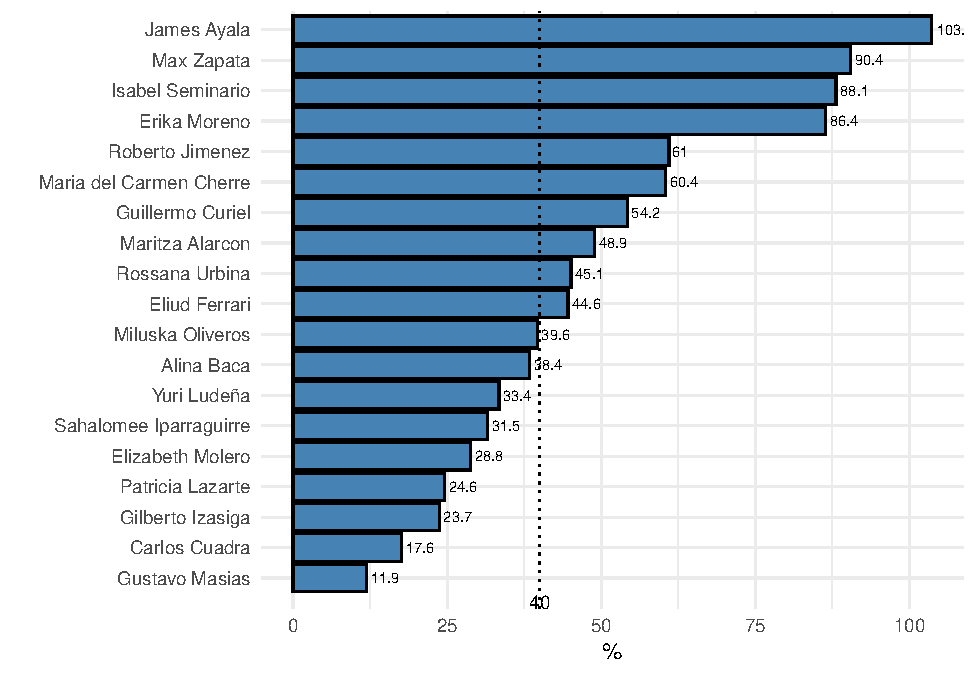
\includegraphics{Journal_files/figure-latex/unnamed-chunk-2-1.pdf}

\hypertarget{analisis-competentencia}{%
\section{Analisis competentencia}\label{analisis-competentencia}}

Y asi se pueden ir agregando mas tablas graficos y conclusiones que se
generan automatico y se cargan a esta web creada para Lansier, a la
izquierda irian apareciendo los nuevos titulos que se asignen conforme
se vayan creando, asi podrian hallar mas rapidamente lo que estan
buscando, esto podria ser un reemplazo del pdf, me comentó que podia ser
una opción para que los jefes no tengan que estar abriendo pdfs cada que
les envio, asi que ahi esta la idea y tal vez se puede modificar algo o
volver al pdf, lo bueno de esta web es que siempre esta online, solo se
necesita el link, es similar a como funciona un dashboard de power bi,
el unico esfuerzo es ejecutra el programa para que actualice la data
jalando del sql y cree el reporte con todo actualizado al igual que
hacemos en el power bi.

\end{document}
